% -*- root: ../Presentation.tex -*-
\section{JPEG indkodning og grafteori}

\begin{frame}{JPEG billede-indkodning}{}
\begin{figure}
\centering
\begin{tikzpicture}[
processnode/.style={rectangle, draw=gray!60, fill=gray!5, very thick, minimum size=4mm,text width=1.5cm, minimum height=2cm},
encodenode/.style={rectangle, dashed,draw=red!60, fill=red!5, very thick, minimum size=4mm,text width=1.5cm, minimum height=2cm},
pre/.style={=stealth',semithick},
post/.style={->,shorten >=1pt,>=stealth',semithick},
]
%Nodes
\node[processnode]        (huffmanencoding)  {Huffman encode quantized values to file};
\node[processnode]        (quantization)     [right=of huffmanencoding] {Quantize the 8x8 blocks};
\node[processnode]        (dct)              [right=of quantization] {Perform DCT on 8x8 blocks from MCU};
\node[processnode]        (sampling)         [above=of dct] {Downsam
ple MCU's};
\node[processnode]        (split)            [left=of sampling] {Split image into MCU's};
\node[processnode]        (convert)          [left=of split] {Convert from RGB to YCbCr};
\node[processnode]        (bitmapimage)      [left=of convert] {\lstinline|Bitmap| \\image};
 
%Lines
\draw[->] (bitmapimage.east) -- (convert.west);
\draw[->] (convert.east) -- (split.west);
\draw[->] (split.east) -- (sampling.west);
\draw[->] (sampling.south) -- (dct.north);
\draw[->] (dct.west) -- (quantization.east);
\draw[->] (quantization.west) -- (huffmanencoding.east);
\end{tikzpicture}
\caption{JPEG indkodning}
\label{fig:JPEGprocess}
\end{figure}
\end{frame}

\begin{frame}{Gemning af data i JPEG billeder}{}
	\begin{minipage}[0.5\textheight]{\textwidth}
		\begin{columns}[T]
			\begin{column}{0.5\textwidth}
				\vspace{.56mm}
				\begin{itemize}
					\item Billede opdeles i MCU'er
					\item Yderligere opdelt i 8x8 blokke
					\item 8x8 blok af integers
				\end{itemize}
			\end{column}
			\begin{column}{0.5\textwidth}
				\begin{center}
					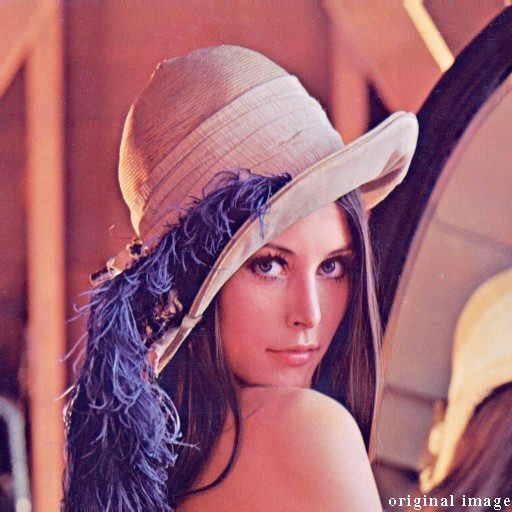
\includegraphics[width=.5\textwidth]{figures/lena_color.jpg}
				\end{center}
				{\tiny \begin{table}[]
						\centering
						\begin{tabular}{|c|c|c|c|c|c|c|c|}
							\hline
							-26 & -3 & -6 & 2  & 2  & -1 & 0 & 0 \\ \hline
							0   & -2 & -4 & 1  & 1  & 0  & 0 & 0 \\ \hline
							-3  & 1  & 5  & -1 & -1 & 0  & 0 & 0 \\ \hline
							-3  & 1  & 2  & -1 & 0  & 0  & 0 & 0 \\ \hline
							0   & 0  & 0  & 0  & 0  & 0  & 0 & 0 \\ \hline
							0   & 0  & 0  & 0  & 0  & 0  & 0 & 0 \\ \hline
							0   & 0  & 0  & 0  & 0  & 0  & 0 & 0 \\ \hline
							0   & 0  & 0  & 0  & 0  & 0  & 0 & 0 \\ \hline
						\end{tabular}
					\end{table}
				}
			\end{column}
		\end{columns}
	\end{minipage}
	\note{
		\begin{itemize}
			\item Meget matematisk billedeformat
			\item Ingen adgang til de enkelte pixels, da de regnes som en fælles block
			\item Starter med en 16x16 block, da vi bruger 4:2:0 sampling $\rightarrow$ 6 8x8 blocks (4 Y, 1 Cb, 1 Cr) $\rightarrow$ DCT $\rightarrow$ quantization $\rightarrow$ huffman encoding $\rightarrow$ skrives til filen (Zero-length entropy).
			\item JPEG encoder lavet til formålet
		\end{itemize}
	}
	
\end{frame}

% -*- root: ../Presentation.tex -*-
\section{Grafteoretisk tilgang til steganografi}
\begin{frame}{Grafteoretisk tilgang til steganografi}{}
	\begin{center}
		
\includegraphics[width=.4\textwidth, frame]{figures/pixelgrid.png}
	\end{center}
	\begin{align*}
		p = \{&106,102,103,100,101,101,200,\\&255,100,125,103,254,104,100\}
	\end{align*}
	$$ e = \{2,2,1,2,1,2,2\} = \{10,10,01,10,01,10,10\}_2$$
	

\end{frame}

\begin{frame}{Grafteoretisk tilgang til steganografi}{}
	$$ x \oplus_m y = (x + y)\mod m $$
	\begin{table}[h]
		\centering
		\resizebox{\textwidth}{!}{%
			\begin{tabular}{|c|c|c|c|c|c|c|c|c|c|c|c|c|c|c|}
				\hline
				Pixels & $p_1$ & $p_2$ & $p_3$ & $p_4$ & $p_5$ & $p_6$ & $p_7$ & $p_8$ & $p_9$ & $p_{10}$ & $p_{11}$ & $p_{12}$ & $p_{13}$ & $p_{14}$ \\ \hline
				Value & 106 & 102 & 103 & 100 & 101 & 101 & 200 & 255 & 100 & 125 & 103 & 254 & 104 & 100 \\ \hline
				$\oplus_4$ & \multicolumn{2}{c|}{0} & \multicolumn{2}{c|}{3} & \multicolumn{2}{c|}{2} & \multicolumn{2}{c|}{3} & \multicolumn{2}{c|}{1} & \multicolumn{2}{c|}{1} & \multicolumn{2}{c|}{0} \\ \hline
				Message & \multicolumn{2}{c|}{2} & \multicolumn{2}{c|}{2} & \multicolumn{2}{c|}{1} & \multicolumn{2}{c|}{2} & \multicolumn{2}{c|}{1} & \multicolumn{2}{c|}{2} & \multicolumn{2}{c|}{2} \\ \hline
				& \multicolumn{2}{c|}{$\neq$} & \multicolumn{2}{c|}{$\neq$} & \multicolumn{2}{c|}{$\neq$} & \multicolumn{2}{c|}{=} & \multicolumn{2}{c|}{=} & \multicolumn{2}{c|}{$\neq$} & \multicolumn{2}{c|}{$\neq$} \\ \hline
				Needed values & \multicolumn{2}{c|}{\begin{tabular}[c]{@{}c@{}}<104,100>\\ <108,104>\end{tabular}} & \multicolumn{2}{c|}{\begin{tabular}[c]{@{}c@{}}<102,99>\\ <106,103>\end{tabular}} & \multicolumn{2}{c|}{\begin{tabular}[c]{@{}c@{}}<100,100>\\ <104,104>\end{tabular}} & \multicolumn{2}{c|}{\begin{tabular}[c]{@{}c@{}}<199,254>\\ <203,002>\end{tabular}} & \multicolumn{2}{c|}{} & \multicolumn{2}{c|}{\begin{tabular}[c]{@{}c@{}}<100,251>\\ <104,255>\end{tabular}} & \multicolumn{2}{c|}{\begin{tabular}[c]{@{}c@{}}<102,98>\\ <106,102>\end{tabular}} \\ \hline
			\end{tabular}%
		}
	\end{table}
	Ombytninger som ville resultere i en forbedring: $(4 \leftrightarrow 11)$, $(8\leftrightarrow 12)$, $(2\leftrightarrow 13)$ and $(1 \leftrightarrow 13)$.
\end{frame}


\begin{frame}{Grafteoretisk tilgang til steganografi}{}
	Fordelagtige ombytninger
	\begin{figure}[h]
		\centering
		\begin {tikzpicture}[-latex ,auto ,node distance =0.6 cm and 0.6cm ,on grid ,
		semithick ,
		state/.style ={ circle ,top color =white ,
			draw , text=black , minimum width =0.3111111111111111 cm},
		state2/.style ={ circle ,color =white ,
			draw , text=black, opacity=0.0 , minimum width =.3 cm}]
		\node[state] (A0) {(1,2)};
		\node[state2] (A1) [right =of A0] {};
		\node[state2] (A2) [right =of A1] {};
		\node[state2] (A3) [right =of A2] {};
		\node[state2] (A4) [right =of A3] {};
		\node[state2] (A5) [right =of A4] {};
		\node[state2] (A6) [right =of A5] {};
		\node[state2] (A7) [right =of A6] {};
		\node[state2] (A8) [right =of A7] {};
		\node[state2] (A9) [right =of A8] {};
		\node[state2] (A10) [below =of A9] {};
		\node[state2] (A11) [below =of A10] {};
		\node[state] (A12) [below =of A11] {(3,4)};
		\node[state2] (A13) [left =of A12] {};
		\node[state2] (A14) [left =of A13] {};
		\node[state2] (A15) [left =of A14] {};
		\node[state2] (A16) [below =of A15] {};
		\node[state2] (A17) [below =of A16] {};
		\node[state] (A18) [below =of A17] {(7,8)};
		\node[state2] (A19) [right =of A18] {};
		\node[state2] (A20) [right =of A19] {};
		\node[state] (A21) [right =of A20] {(11,12)};
		\node[state2] (A22) [left =of A21] {};
		\node[state2] (A23) [left =of A22] {};
		\node[state2] (A24) [left =of A23] {};
		\node[state2] (A25) [left =of A24] {};
		\node[state2] (A26) [left =of A25] {};
		\node[state] (A27) [left =of A26] {(13,14)};
		\path[-] (A12) edge node[] {$4 \leftrightarrow 11$}(A21);
		\path[-] (A18) edge node[right=-.6cm,above=.6cm] {$8\leftrightarrow 12$}(A21);
		\path[-] (A0) edge [bend right =-45] node[] {$2\leftrightarrow 13$}(A27);
		\path[-] (A0) edge [bend right =45] node[] {$1 \leftrightarrow 13$}(A27);
	\end{tikzpicture}
\end{figure}


\note{Der kunne tilføjes kantvægt for bedre parring, så der kom mindst mulig ændring}
\end{frame}

\begin{frame}{Grafteoretisk tilgang til steganografi}{}
	\begin{table}[h]
		\centering
		\resizebox{\textwidth}{!}{%
			\begin{tabular}{|c|c|c|c|c|c|c|c|c|c|c|c|c|c|c|}
				\hline
				Pixels & $p_1$ & $p_2$ & $p_3$ & $p_4$ & $p_5$ & $p_6$ & $p_7$ & $p_8$ & $p_9$ & $p_{10}$ & $p_{11}$ & $p_{12}$ & $p_{13}$ & $p_{14}$ \\ \hline
				Value & 106 & 104 & 103 & 103 & 101 & 101 & 200 & 255 & 100 & 125 & 100 & 254 & 102 & 100 \\ \hline
				$\oplus_4$ & \multicolumn{2}{c|}{2} & \multicolumn{2}{c|}{2} & \multicolumn{2}{c|}{2} & \multicolumn{2}{c|}{3} & \multicolumn{2}{c|}{1} & \multicolumn{2}{c|}{2} & \multicolumn{2}{c|}{2} \\ \hline
				Message & \multicolumn{2}{c|}{2} & \multicolumn{2}{c|}{2} & \multicolumn{2}{c|}{1} & \multicolumn{2}{c|}{2} & \multicolumn{2}{c|}{1} & \multicolumn{2}{c|}{2} & \multicolumn{2}{c|}{2} \\ \hline
				& \multicolumn{2}{c|}{=} & \multicolumn{2}{c|}{=} & \multicolumn{2}{c|}{$\neq$} & \multicolumn{2}{c|}{=} & \multicolumn{2}{c|}{=} & \multicolumn{2}{c|}{=} & \multicolumn{2}{c|}{=} \\ \hline
				Needed values & \multicolumn{2}{c|}{} & \multicolumn{2}{c|}{} & \multicolumn{2}{c|}{\begin{tabular}[c]{@{}c@{}}<100,100>\\ <104,104>\end{tabular}} & \multicolumn{2}{c|}{} & \multicolumn{2}{c|}{} & \multicolumn{2}{c|}{} & \multicolumn{2}{c|}{} \\ \hline
			\end{tabular}%
		}
	\end{table}
	\begin{figure}
\centering     %%% not \center
\subfigure[]{
\includegraphics[width=.4\textwidth,frame]{figures/pixelgrid.png}}
\subfigure[]{
\includegraphics[width=.4\textwidth,frame]{figures/pixelgrid2.png}}
\caption{Billede før og efter GT}
\end{figure}
\end{frame}